\documentclass{beamer}
\usepackage{pgf}
\usepackage{amsmath}
\usepackage{multirow}
\usepackage{setspace}
\usepackage{threeparttable}
\usepackage[english]{babel}
\usepackage{multimedia}
\usepackage{hyperref}
\usepackage{epstopdf}
\usepackage{subfigure}
\usepackage{graphicx}
\usepackage{scalefnt}
\usepackage{tikz}
\usepackage{eepic}

\DeclareMathOperator*{\plim}{plim}

\newcommand{\highlight}[1]{\colorbox{yellow}{$\displaystyle #1$}}

\newcommand{\bfhat}[1]{\hat{\boldsymbol{#1}}}

\newcommand\independent{\protect\mathpalette{\protect\independenT}{\perp}}
\def\independenT#1#2{\mathrel{\rlap{$#1#2$}\mkern2mu{#1#2}}}

\mode<presentation>
{
\setbeamercovered{transparent}
\usetheme{CambridgeUS}
\usecolortheme{dolphin}
}
\setbeamertemplate{button}{\tikz
  \node[
  inner xsep=10pt,
  draw=structure!80,
  fill=structure!50,
  rounded corners=4pt]  {\Large\insertbuttontext};}

\setbeamertemplate{section page}
{
    \begin{centering}
    \begin{beamercolorbox}[sep=12pt,center]{part title}
    \usebeamerfont{section title}\insertsection\par
    \end{beamercolorbox}
    \end{centering}
}

\title{Introduction}

\begin{document}
\maketitle

\begin{frame}{Overview}
\tableofcontents
\end{frame}

\section{Why Economics of Education?}
\begin{frame}{Why Study Education?}
Simple answer:   
   \begin{itemize}
       \item We spend over \$ 1.2 trillion on education in the United States. 
       \item Majority of economic output comes from labor
       \item Schools are thought to play an important role in training labor force
   \end{itemize}
Not so simple answer:
    \begin{itemize}
        \item Schools play an important role in students lives and in society
        \item Goals of education are multi-dimensional
        \item Education in the US involves a complex mix of problems and decisions at the individual level (e.g. students and teachers), organizational level (schools and districts), and political level (departments of education, governing bodies)
        \item Education, like many social policy arenas, has a history of ongoing issues of inequality
    \end{itemize}
\end{frame}

\begin{frame}{Why Study Economics of Education}
Alright, but why the economics of education?    
    \begin{itemize}
        \item There are certainly other theories and methods that provide useful insights into education policy topics. But in this class we focus on the use of economics. 
        \item Economic theories provide useful models to understand how individuals make decisions. For example, they help us understand: 
        \begin{itemize}
            \item how students and families choose schools
            \item how peers influence student outcomes
            \item who becomes a teacher and where do they choose to work
            \item how to design policies that hold teachers and schools accountable for student outcomes
            \item and so on ...
        \end{itemize}
        \item Economists have also pushed the methodological envelope by refining and designing statistical techniques to estimate the causal impact of social policies and programs.
    \end{itemize}
\end{frame}
\begin{frame}{Important Economic Principles}
Although a review for you, we will see a few classic economic ideas re-occur throughout the readings
    \begin{itemize}
        \item Scarcity
        \item Opportunity Costs
        \item Budget Constraints
        \item Trade-offs
        \item Diminishing Marginal Returns
    \end{itemize}
\end{frame}

\begin{frame}{Important Economic Principles}
As mentioned in the book, economics tools and theories help us think about
    \begin{itemize}
        \item What should be produced
        \item How much should we produce
        \item And for whom should it be produced?
    \end{itemize}
\end{frame}    

\begin{frame}{Important Building Blocks}
    In this class we will often talk about two key components of education policy and research    
    \begin{itemize}
        \item \textbf{Inputs}: Any factors or resources that contribute to building an individual's ability or knowledge
        \begin{itemize}
            \item Some inputs are both easy to measure and change with policies and/or incentivize (e.g. class-size, textbooks)
            \item Other inputs we're starting to measure better but are hard to change with policy (e.g. teacher quality)
            \item Others yet are both hard to measure and hard to change with policy (e.g. peers, neighborhoods, building quality)
        \end{itemize}
        \item \textbf{Outputs}: Any knowledge, skill, or attribute that is a result of participation in the education process
        	\begin{itemize}
		\item Often there's two (or more) dimensions to the outputs of interest:
      	  	\begin{itemize}
        	  		 \item The amount of \textbf{time} that has lapsed since the exposure to a policy/practice/incentive of interest
        	   	 	\item The \textbf{specificity} of the output (e.g. multiplication of two-digit integers versus broader civic behavior).
        		\end{itemize}
	\end{itemize}	
    \end{itemize}
\end{frame}    

\begin{frame}{Types of Education Policies}
In this class we will read about three broad types of policies
    \begin{itemize}
        \item \textbf{Total Resource Policies} which increase the total amount of funding to schools (interestingly this is one of the most contentious literatures in education research)
        \item \textbf{Input-based policies} which focus on specific inputs such as class-size, teaching credentials, length of the school year. These were quite popular through NCLB. 
        \item \textbf{Output-based policies} which tie the performance of students, teachers, or schools (or other entities) to incentives (e.g. rewards/sanctions). The use of these policies has exploded in the past 10 years.   
    \end{itemize}
\medskip
In short, most policies can be seen as a set of incentives. Incentives often change behavior, but an important question is whether the behavioral change(s) was intended and the net effect was in the anticipated direction. 
    
\end{frame}

\begin{frame}{Markets in Education}
Education is a unique marketplace:    
    \begin{itemize}
        \item It is not perfectly competitive (e.g. typically large start up costs, imperfect information)
        \item Spillovers or externalities are quite common (we'll a number of interesting papers on this topic). 
        \item Supply is often local, but this is changing with the use of virtual education
        \item Education is highly differentiated, both vertically (age) and horizontally (flavors of education for a given age)
        \item The quality of your education is influenced by the characteristics of other consumers (peers)
    \end{itemize}
\medskip
However a number of interesting education policies are based on near perfectly competitive market principles (e.g. school choice). We'll read about what happens in these settings.
\end{frame}

\begin{frame}{Why Does the US Gov Participate in Education?}
    \begin{itemize}
        \item Education is a consumption good. The market for consumption goods (movies, wine, education) generally has some degree of information asymmetry.
        \item Education often benefits from economics of scale (e.g. why is there a negative correlation between high school size and the \# of AP classes offered?)
        \item Education has positive externalities, and in these cases people typically under consume goods. 
        \item Individuals differ in their budget constraints which affects their ability to access credit. 
    \end{itemize}
    
\end{frame}

\section{Bias}
\frame{\sectionpage}


\begin{frame}{Bias - The Difference Between Causal and Correlational}
\begin{itemize}
    \item In this class we will spend A LOT of time talking about the effect of policies/practice/interventions on a variety of outcomes.
    \item In order to talk about \textbf{effects}, we need to be fairly certain we've isolated causal relationships
    \item The extent to which an estimated impact is expected to differ from the true impact is statistical \textit{bias}.
    \item In essences it is the difference between the measured correlation and the actual causal impact.

\end{itemize}
\end{frame}

\begin{frame}{Why Do We Need to Know Causal Information?}
    \begin{itemize}
        \item Much of microeconometrics today involves the pursuit of \textit{causal inference}.
        \begin{itemize}
            \item The ability to establish a causal relationship between two factors.
            \item This is opposed to \textit{correlation} which is an estimate of a statistical relationship between two factors.
        \end{itemize}
        \item Consider the following example
            \begin{itemize}
                \item A matter of much controversy in educating English Language Learners (ELLs) is whether it is better to provide immersive English instruction or a bilingual instructional environment.
                \item How can one figure out which is better?
                \item Tempting to simply compare students in English immersion to those in bilingual education.
            \end{itemize}
        \end{itemize}
 \end{frame}

\begin{frame}{Bad Causality Leads to Bad Policy}
\begin{itemize}
    \item It's clear from a statistical perspective we want to get to the ``truth.'' \bigskip
    \item But from a practical perspective why is this so important?  So what if we are off a bit in the policy impact estimates? \bigskip
    \item What's the worst that can happen?
\end{itemize}
\end{frame}

\begin{frame}{Formula for OLS Coefficients}
    \begin{itemize}
        \item Remember the formula for an OLS regression coefficient
 	\item The simple algebra formula for a single regression coefficient is
	        \begin{equation}
            		\hat{\beta} = \frac{cov(X,Y)}{var(X)}
        		\end{equation}
        
        \item The matrix algebra formula for multiple regression coefficients is	
       \begin{equation}
            \bfhat{\beta} = \mathbf{\frac{X'Y}{X'X}} = \left(\mathbf{X'X}\right)^{-1}\mathbf{X'Y}
        \end{equation}
    \end{itemize}
\end{frame}


\begin{frame}{Consistency vs. Unbiasedness}
    \begin{itemize}
        \item While consistency and unbiasedness are technically distinct, an unbiased estimator is almost always consistent (and will be consistent in any context we learn in this class). \medskip
        \item Thus our focus today (and mostly in your readings as well) will be more on unbiasedness. \medskip
        \item Before we talk about when an OLS estimate is unbiased, let's talk through a thought experiment from our textbook: ability bias in our estimated relationship between earnings and education. 
    \end{itemize}
\end{frame}

\begin{frame}{Ability Bias}
    \begin{itemize}
        \item Many studies find a positive a positive relationship between education and labor productivity. \medskip
        \item Does this mean that our simple bivariate regression coefficient ($\hat{\beta}$) represents a causal estimate of the returns to education? 
        \begin{itemize}
        		\item Are there other factors that are both correlated with education and labor market productivity?
        \end{itemize}
        \item The answer to this question has important implications to how we may design future education policies.  
    \end{itemize}
\end{frame}

\begin{frame}{Ability Bias}
    \begin{itemize}
        \item Let's take ability as an example of a factor related to both years of education and labor market productivity. 
        \item In most scenarios, we have to rely on proxies for ability, in this case individuals' SAT scores.  
       	\item It is likely that higher ability people not only are more likely to extend their education, but are also likely to earn more in the labor market. 
	\item If this is true, our simple bivariate regression coefficient then includes both the true return to education as well as the impact of ability on earnings. 
    \end{itemize}
\end{frame}

\begin{frame}
\begin{columns}
	\begin{column}{0.48\textwidth}
	    \begin{figure}[h]
    		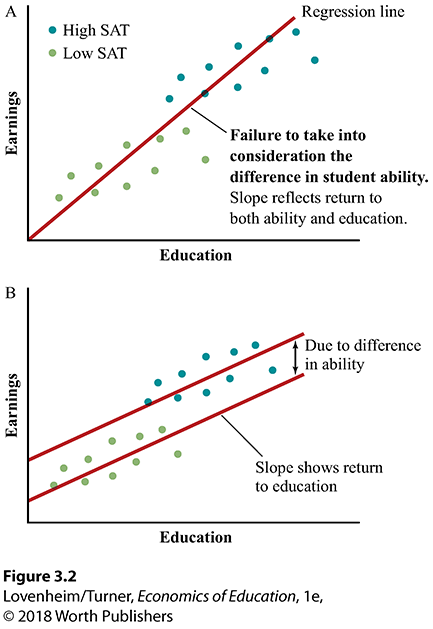
\includegraphics[width = 2.15in]{turner1e_fig_03_02.png}
   	 \end{figure}
	\end{column}
	\begin{column}{0.48\textwidth}
		\begin{itemize}
			\item The Figures show that for the same education level, individuals with higher ability earn more than individuals with lower ability \bigskip
			\item We also see that the true returns to education (Figure B) is flatter than the biased estimate in Figure A
		\end{itemize}
		
	\end{column}
\end{columns}


\end{frame}

\begin{frame}{When is OLS unbiased?}
    \begin{itemize}
        \item There are a few conditions under which we can assume that OLS is unbiased.
    \end{itemize}
    \begin{enumerate}
        \item The model is of the correct functional form \begin{itemize}\footnotesize
                 \item This just means that we have correctly specified the model, e.g. that we include the correct variables and that they are in the model in the appropriate fashion (e.g. $x$, $x^2$, $xz$, etc). \medskip
                 \item This also implies that the true model is linearly additive.  That is, it has the form $y = \beta_0 + \beta_1x_1 + ... + \beta_kx_k + \varepsilon$ instead of something nonlinear like $y = \beta_0x^{\beta_1}\varepsilon$. \medskip
                 \item In practice, in economics of education research tends to use additively linear models and this is a routine assumption.
            \end{itemize}
      \end{enumerate}
\end{frame}

\begin{frame}{When is OLS unbiased?}
    \begin{enumerate}
        \setcounter{enumi}{1}
        \item All independent variables are linearly independent.
            \begin{itemize} \footnotesize
                \item Basically this says that no set of variables in the regression can come together in the form $x_0 = b_0 + b_1x_1 + ... + b_jx_j.$
                \item In practice you do not need to worry much about this as most statistical programs will take care of this for you by dropping one of the variables.
                \item Most often this occurs when you have a mutually exclusive categorical variable.
                \item For example say you want to regress test scores on race, where race can be black, white or other $\rightarrow Black_i = 0/1; White_i = 0/1; Other_i = 0/1$ where only one category can equal 1 for a person.
                    \begin{equation*}
                       Score_i = \beta_0 + \beta_1White_i + \beta_2Black_i + \beta_3Other_i + \varepsilon
                    \end{equation*}

                    is not permissible. Instead you would estimate

                    \begin{equation*}
                       Score_i = \beta_0 + \beta_1White_i + \beta_2Black_i + \varepsilon
                    \end{equation*}

                    and $\beta_1$ will be the relationship between test scores and being black \textit{relative} to other, and similarly for $\beta_2$ and white.
                \end{itemize}
        \end{enumerate}
\end{frame}

\setcounter{equation}{4}
\begin{frame}{When is OLS unbiased?}
    \begin{enumerate}
        \setcounter{enumi}{2}
        \item The third and most important assumption is that the independent variables $X$ are exogenous - they are uncorrelated with $\varepsilon$.

            \begin{itemize}
            \item This leads to the following condition
                \begin{equation}
                E(\boldsymbol{\varepsilon}|\mathbf{X} ) = 0
                \end{equation}  \label{exogeneity}

            \item This says that conditional on the $X$ the error terms have expected values of 0. This is also sometimes called the ``exogeneity assumption.''

            \item This condition also holds if and only if  the covariance of each $x_j$ with $\varepsilon$ is zero:

                 \begin{equation}
                 Cov(x_j, \varepsilon) = 0
                \end{equation}

            \item Note that if $\varepsilon$ is normally distributed with a mean of 0, the exogeneity condition holds.
		
            \end{itemize}
  \end{enumerate}
\end{frame}


\begin{frame}{What happens when the Exogeneity Condition Doesn't Hold?}
	\begin{itemize}
		\item Let's assume that an individual's outcome $Y_{i}$ is a function of her years of education ($Ed_i$) and ability ($Ability_i$)
      		  \begin{equation}
        			Y_{i}=\beta_0+\beta_{1}Ed_{i} +\beta_{2}Ability_{i} +\epsilon
       		 \end{equation}
		     \pause
		 \item What happens if we just estimate our original model, omitting ability?
      		  \begin{equation}
        			Y_{i}=\gamma_0+\gamma_{1}Ed_{i} +\mu
       		 \end{equation}		
		     \pause
		\item Using our formula for a regression coefficient  $E(\hat{\gamma_1})=\frac{cov(Y,Ed_i)}{var(Ed_i)}$, and substituting $\alpha+\beta_{1}Ed_{i} +\beta_{2}Ability_{i} +\epsilon$ for $Y_i$, we get:
		 \begin{equation}
        			E(\hat{\gamma_1})=\frac{cov(\alpha+\beta_{1}Ed_{i} +\beta_{2}Ability_{i} +\epsilon,Ed_i)}{var(Ed_i)}
       		 \end{equation}	

	\end{itemize}

\end{frame}

\begin{frame}{What happens when the Exogeneity Condition Doesn't Hold?}
	\begin{equation}
        		=\frac{cov(\beta_0,Ed_i)}{var(Ed_i)}+\beta_1 +\beta_{2}\frac{cov(Ability_i,Ed_i)}{var(Ed_i)}+\frac{cov(\epsilon, Ed_i)}{var(Ed_i)}
       	\end{equation}	

	\begin{itemize}
		\item The first term is zero since $\beta_0$ is a constant and the last term is also zero given the main OLS assumptions ($cov(\epsilon, X_i)=0$)
		\pause
		\item This leaves us with the omitted variable bias formula:
	\begin{equation}
        		E(\hat{\gamma_1})=+\beta_1 +\beta_{2}\frac{cov(Ability_i,Ed_i)}{var(Ed_i)}
       	\end{equation}	
	\pause	
	\item Note that the last term $\frac{cov(Ability_i,Ed_i)}{var(Ed_i)}$ is the coefficient from a bivariate regression of $Ability_i$ on $Ed_i$
	\item OVB is driven by factor(s) that are more correlated with your independent variables of interest and your dependent variable. 
	\end{itemize}

\end{frame}

\begin{frame}{What happens when the Exogeneity Condition Doesn't Hold?}
	\begin{itemize}
		\item We are left with two options to deal with selection or omitted variable bias
		\begin{enumerate}
			\item Include all of the variables in our OLS regression that are related to treatment and outcome (very difficult to do in practice) \medskip
			\item Find a source of exogenous variation in the treatment variable that removes selection bias from our statistical analysis
		\end{enumerate} 
	\item  Throughout the course we will now discuss common methods used to find exogenous variation in treatment assignment. We will provide refreshers for the methods as they come up in the readings. We can also suggest a number of useful books to use as a reference (e.g Mostly Harmless Econometrics). 
	
	\end{itemize}

\end{frame}

\end{document}